\subsection{GSM2}
\selectlanguage{russian}

Регистрация телефона в сети GSM2 построена с участием трех сторон: сим-карты мобильного устройства, базовой станции и центра аутентификации. Сим-карта и центр аутентификации обладают общим секретным 128-битовым ключом $K_i$. Вначале телефон сообщает базовой станции уникальный идентификатор сим-карты IMSI открытым текстом. Базовая станция запрашивает в Центре аутентификации для данного IMSI набор параметров для аутентификации. Центр генерирует псевдослучайное 128-битовое число $\textrm{RAND}$ и алгоритмами A3 и A8\index{алгоритм!A3, A5, A8} создает симметричный 54-битовый ключ $K_c$ и 32-битовый аутентификатор $\textrm{RES}$. Базовая станция передает мобильному устройству число $\textrm{RAND}$ и ожидает результат вычисления сим-картой числа $\textrm{XRES}$, которое должно совпадать с $\textrm{RES}$ в случае успешной аутентификации. Схема аутентификации показана на рис. \ref{fig:gsm2}.

\begin{figure}[h!]
	\centering
	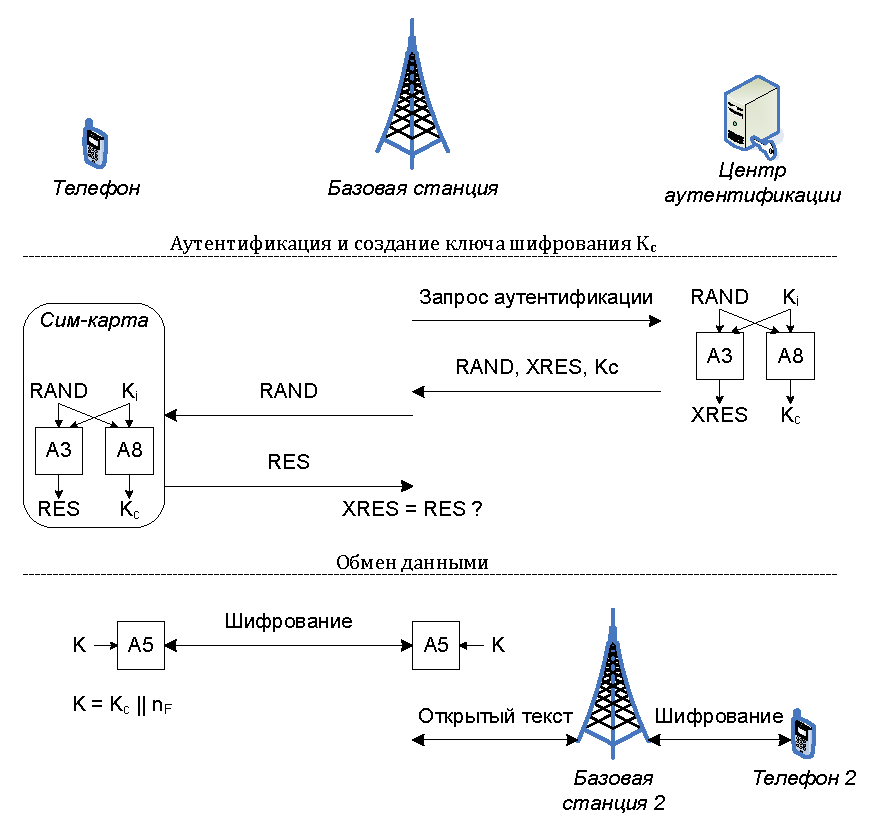
\includegraphics[width=0.85\textwidth]{pic/gsm2}
	\caption{Односторонняя аутентификация и шифрование в GSM2\label{fig:gsm2}}
\end{figure}

Все вычисления для аутентификации выполняет сим-карта. Ключ $K_c$ далее используется для создания ключа шифрования каждого фрейма $K = K_c \| n_F$, где $n_F$ -- 22-битовый номер фрейма. Шифрование выполняет уже само мобильное устройство. Алгоритм шифрования фиксирован в каждой стране и выбирается из семейства алгоритмов A5 (A5/1, A5/2, A5/3). В GSM2 применяется либо алгоритм A5/1, либо A5/2 (используется в России). Алгоритм A5/3 применяется уже в сети GSM3.

Аутентификация в сети GSM2 односторонняя. При передаче данных не используются проверка целостности и аутентификация сообщений. Передача данных между базовыми станциями происходит в открытом незашифрованном виде. Алгоритмы шифрования A5/1 и A5/2 не стойкие, количество операций для взлома A5/1 -- $2^{40}$, A5/2 -- $2^{16}$. Кроме того, длина ключа $K_c$ всего 54 бита. Передача в открытом виде уникального идентификатора IMSI позволяет однозначно определить абонента.
